% $Header$

\documentclass{beamer}

% This file is a solution template for:

% - Giving a talk on some subject.
% - The talk is between 15min and 45min long.
% - Style is ornate.



% Copyright 2004 by Till Tantau <tantau@users.sourceforge.net>.
%
% In principle, this file can be redistributed and/or modified under
% the terms of the GNU Public License, version 2.
%
% However, this file is supposed to be a template to be modified
% for your own needs. For this reason, if you use this file as a
% template and not specifically distribute it as part of a another
% package/program, I grant the extra permission to freely copy and
% modify this file as you see fit and even to delete this copyright
% notice. 


\mode<presentation>
{
  %\usetheme{Warsaw}
  %\usetheme{Berlin}
  %\usetheme{metropolis}
  \usetheme{PaloAlto}
  %\usetheme{CambridgeUS}
  %\usetheme{Berkeley}
  
  % font themes
  \usefonttheme{serif}
  %\usefonttheme{structurebold}

  % color themes
  %\usecolortheme{albatross}
  %\usecolortheme{beetle}
  %\usecolortheme{crane}
  %\usecolortheme{dove}
  %\usecolortheme{fly}
  %\usecolortheme{monarca}
  %\usecolortheme{seagull}
  %\usecolortheme{beaver}
  % color themes
  % or ...

  %\setbeamercovered{transparent}
  \setbeamercovered{transparent=5}
  % or whatever (possibly just delete it)
}


\usepackage[english]{babel}
% Place figures exactly where you mean to
%https://tex.stackexchange.com/a/8633/64425
\usepackage{float}
% Place figures exactly where you mean to
% or whatever

\usepackage[utf8]{inputenc}
% or whatever

\usepackage[T1]{fontenc}
% Or whatever. Note that the encoding and the font should match. If T1
% does not look nice, try deleting the line with the fontenc.

% math
\usepackage{amsmath}
\usepackage{amssymb}
\usepackage{amsthm}
% math

% tikz
\usepackage{tikz}
% tikz
\usepackage{caption}
\usepackage{hyperref}
\hypersetup{
    colorlinks,
    linkcolor={magenta!50!black},
    citecolor={blue!50!black},
    urlcolor={blue!80!black}
}
% large commented sections
\usepackage{comment}
% large commented sections



\title[Getting Started with Calculus] % (optional, use only with long paper titles)
{Learning Calculus from the Masters}

\subtitle
{How to Build on Elementary Ideas} % (optional)

\author[Augustus De Morgan, Thomas McCormack, KM] % (optional, use only with lots of authors)
{A.~De Morgan\inst{1} \and T.~McCormack\inst{2}}
% - Use the \inst{?} command only if the authors have different
%   affiliation.

\institute[SDUK] % (optional, but mostly needed)
{
  \inst{1}%
  Original Author
  \and
  \inst{2}%
  First Maintainer
  }
% - Use the \inst command only if there are several affiliations.
% - Keep it simple, no one is interested in your street address.

\date[August 2025] % (optional)
{Aug 2025 / Free Learner's School Conversations}

\subject{Fun Conversations at Home School}
% This is only inserted into the PDF information catalog. Can be left
% out. 



% If you have a file called "university-logo-filename.xxx", where xxx
% is a graphic format that can be processed by latex or pdflatex,
% resp., then you can add a logo as follows:

% \pgfdeclareimage[height=0.5cm]{university-logo}{university-logo-filename}
% \logo{\pgfuseimage{university-logo}}



% Delete this, if you do not want the table of contents to pop up at
% the beginning of each subsection:
\AtBeginSubsection[]
{
  \begin{frame}<beamer>{Outline}
    \tableofcontents[currentsection,currentsubsection]
  \end{frame}
}


% If you wish to uncover everything in a step-wise fashion, uncomment
% the following command: 

%\beamerdefaultoverlayspecification{<+->}


\begin{document}

\begin{frame}
  \titlepage
\end{frame}

\begin{frame}{Outline}
  \tableofcontents
  % You might wish to add the option [pausesections]
\end{frame}


% Since this a solution template for a generic talk, very little can
% be said about how it should be structured. However, the talk length
% of between 15min and 45min and the theme suggest that you stick to
% the following rules:  

% - Exactly two or three sections (other than the summary).
% - At *most* three subsections per section.
% - Talk about 30s to 2min per frame. So there should be between about
%   15 and 30 frames, all told.

% [Kedar] I am keeping this structure, but abusing it to serve my purpose.
% [Kedar] I expect this `presentation' to have many hundred slides, if I end up doing it right.
% [Kedar] There are three sections per presentation, no subsections, but each section may have many, many slides. Let's see. I am just getting started with LaTeX and Beamer.
% [Kedar] I may roughly make a chapter in his book a section in this presentation.
\section{Introduction}

%\subsection[The Beginning]{First Subsection Name}

\begin{frame}
%[standout] available only in the `moloch' theme
\frametitle{Learn from the Masters}
{\Large WE LEARN FROM THE MASTERS.}
\end{frame}

\begin{frame}
\frametitle{Learn from the Masters}
WHY?
\end{frame}
\begin{frame}
\frametitle{Learn from the Masters}
\begin{itemize}
\pause
\item Masters May Seem Austere And Sound Cryptic, \pause But They Have Two Essential Traits
\pause
\begin{itemize}
\item Kindness 
\item Dependable and Thorough Knowledge of Something
\end{itemize}
\pause
\item They Want You to Know What They Do (Know)
\pause
\item They Understand Your Difficulties and Sympathize with You
\pause
\item They Are Gentle, But \emph{Don't} Dumb Down The Subject Matter
\end{itemize}
\end{frame}

\begin{frame}
%[standout] available only in the `moloch' theme
\frametitle{Learn from the Masters}
THAT'S WHY.
\end{frame}

\begin{frame}
\frametitle{Learn from the Masters}
\begin{figure}[H]
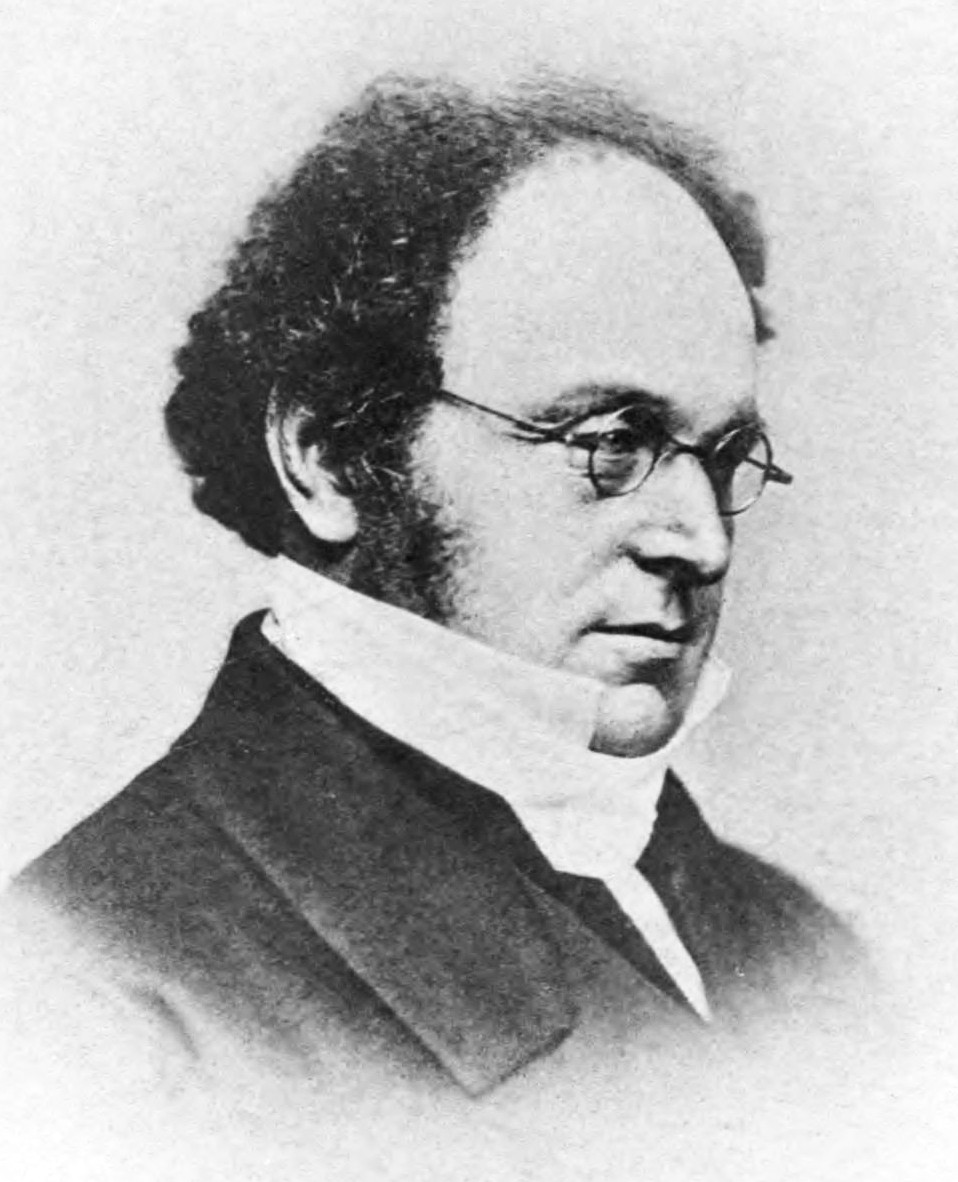
\includegraphics[width=.345\textwidth]{images/de-morgan}
\caption{Augustus De Morgan Was A Master}
\label{fig:de-morgan}
\end{figure}
\end{frame}

\begin{frame}
\frametitle{Learn from the Masters}
He Was A Great Mathematician Interested in Math Education, And He Wrote Several Books to Help Students Learn Math on Their Own!

Here Is a Tiny Story about Him:
\pause

\hrulefill

{\small
Someone asked De Morgan, who lived in the 1800s, ``Dear Mr. De Morgan, in which year were you born?'' 

De Morgan replied, ``I was $x$ years old in the year $x^2$. In which year was I born?''
}

\hrulefill

\pause

Which Year? :-)

\end{frame}

\begin{frame}
\frametitle{Learn From The Masters}

DON'T WE WANT TO LEARN FROM SUCH A MASTER?
\end{frame}

\section{Ratio and Proportion of Two Magnitudes}

\begin{frame}
%[standout] available only in the `moloch' theme
\frametitle{Lest We Forget \dots}
\begin{itemize}
\item 
Reminder:
In Mathematics, As in Everyday Speech, Words are Important.
We Must Understand Them Precisely in The Given Context.
\pause
\item
Problem:
Mathematics Uses Common Words and Gives Them Meanings That May Be Confusing at First.
\end{itemize}
\end{frame}

\begin{frame}
\frametitle{Lest We Forget \dots}
\begin{itemize}
\item Some Words of Mathematics are ``Definitions''.
\pause
\item Be Patient. 
\pause
\item Ask Sincere Questions Till They Are Clear.
\end{itemize}
\end{frame}

\begin{frame}
\frametitle{Commensurable}
Here Is A Definition!
\pause
\begin{definition}[Commensurable]
Two Magnitudes or Lengths or Measures Are Commensurable If They Can Be Expressed in Whole Numbers of Some Common Unit.
\label{def:commensurable}
\end{definition}

{\tiny To Recap [\ref{slide:commensurablerecap}]}
{\tiny To Modern Language [\ref{slide:modernlanguage}]}

\pause
Note: The Common Unit Can Be Made As Small or As Big As We Please.

\pause

Note: Mensurable Means Measurable.
\end{frame}

\begin{frame}
\frametitle{Commensurable}
That Is a Mouthful,

\pause 

And Sounds Complicated!

\pause

But We Can Deconstruct it Slowly \dots
\end{frame}

\begin{frame}
\frametitle{Example: Commensurable}
Consider An Example!
\begin{example}
`Foot' and `Yard' Are Units of Length.

\pause

1 Foot is \textbf{Commensurable} with 1 Yard. 

\pause

1 Foot = 12 Inches and 1 Yard = 36 Inches
\pause
\begin{itemize}
\item If the ``Common Unit'' is 3 (Inches), then 1 Foot Is \textbf{4} Common Units and 1 Yard Is \textbf{12} Common Units. Both 4 and 12 are Whole Numbers.
\pause
\item If the ``Common Unit'' is 6 (Inches), then 1 Foot Is \textbf{2} Common Units and 1 Yard = \textbf{6} Common Units. Both 2 and 6 are Whole Numbers.
\pause
\item If the ``Common Unit'' is 1 (Inch), then 1 Foot Is \textbf{12} Common Units and 1 Yard Is \textbf{36} Common Units. Both 12 and 36 are Whole Numbers.
\pause
\end{itemize}
\end{example}
\end{frame}

\begin{frame}
\frametitle{Example: Commensurable}
We \textit{Showed} That, with A Choice of 3 Common Units
\footnote{Although the Definition Requires Just One},

\pause

(The Lengths) 1 Foot and 1 Yard Are Commensurable.
\end{frame}

\begin{frame}
\frametitle{Example: Commensurable}
Consider Another Example!
\begin{example}
SFO $\rightarrow$ NYC is a 6-Hour Flight.\\
SFO $\rightarrow$ DTW is a $5\frac{1}{2}$-Hour Flight.

Are These Two Periods, or Lengths of Time: $T_1=6,T_2=5\frac{1}{2}$, Commensurable?
\pause
\begin{itemize}
\item What is Your Common Unit?
\pause
\item How Many Whole Numbers of That Common Unit Are $T_1,T_2$?
\end{itemize}
\end{example}
\end{frame}

\begin{frame}
\frametitle{Example: Commensurable}

Very Well Then! 

\pause

To Show That Two Lengths Are Commensurable, We Find A Common Unit and Demonstrate That Each Length Equals Some Whole Number Times It.
\end{frame}

\begin{frame}
\frametitle{Example: Commensurable}

You Are Convinced That $T_1=6,T_2=5\frac{1}{2}$ Are Commensurable, Right?

\end{frame}




\begin{frame}
\frametitle{Why Lengths?}
We Say `Lengths' Because Humanity Measured Things Since Antiquity.

\pause

We Also Say `Magnitudes'.

\pause

Like In Everyday Language, We Use `Length' and `Magnitude' \textit{Synonymously}.

\pause

Geometry Played A Big Role in Our Understanding of Mathematics \dots
\end{frame}

\begin{frame}
\frametitle{Examples And Counterexamples}

We Saw 2 `Examples' of Commensurable Magnitudes.

Sometimes, However, Counterexamples Are Helpful Too.

\pause

Are There Lengths That Are \alert{Not} Commensurable?

\end{frame}


\begin{frame}
\frametitle{Commensurable Or Not?}

\pause

\begin{figure}
\centering
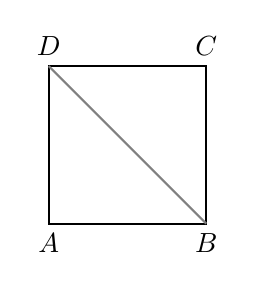
\begin{tikzpicture}[baseline=4mm]
\def\s{2}
\draw[thick] (0,0) -- (\s,0) -- (\s,\s) -- (0,\s) -- cycle;
\draw[thick,gray] (0,\s) -- (\s,0);
\coordinate (A) at (0,0);
\coordinate (B) at (\s,0);
\coordinate (C) at (\s,\s);
\coordinate (D) at (0,\s);
\draw[thick] (A) node [anchor=north] {\(A\)} -- cycle;
\draw[thick] (B) node [anchor=north] {\(B\)} -- cycle;
\draw[thick] (C) node [anchor=south] {\(C\)} -- cycle;
\draw[thick] (D) node [anchor=south] {\(D\)} -- cycle;
\end{tikzpicture}
\caption{A Unit Square}
\label{fig:unitsq}
\end{figure}

In the Unit Square ABCD, 

Are Its Side (\pause e.g. AB) and Its Diagonal (\pause e.g. BD) Commensurable?

\end{frame}


\begin{frame}
\frametitle{Commensurable Or Not?}

In The Square ABCD [\ref{fig:unitsq}], 
\pause
\[
l(AB)=1, l(BD)=\sqrt{1^2+1^2}=\sqrt{2}
\]
\pause
(From The Pythagorean Theorem).

\end{frame}


\begin{frame}
\frametitle{Commensurable Or Not?}

\begin{itemize}
\item It Turns out That \alert{$1$ and $\sqrt{2}$ Are Not Commensurable}!
\pause
\item There's \alert{No Common Unit}, However Small, Of Which $1$ and $\sqrt{2}$ Are Both Whole Numbers!
\end{itemize}
\end{frame}


\begin{frame}
\frametitle{Incommensurable?}

\begin{itemize}
\item We Repeat, \alert{To Show That Commensurable Lengths \pause(e.g. $2.1$, $17.8$) \pause Are Indeed So \dots}
\pause
\begin{itemize}
\item We \textit{Creatively} Find A Common Unit \pause(e.g. $0.1$), And
\pause
\item Demonstrate That The Lengths Are Its Whole Numbers \pause(e.g. $21\in\mathbb{Z}$ and $178\in\mathbb{Z}$ respectively).
\end{itemize}
\pause
\item Will That Approach Work \alert{To Show That Incommensurable Lengths \pause(e.g. $\sqrt[3]{3},\sqrt[4]{5}$) Are Indeed So}? 
\begin{itemize}
\pause
\item That Will Be An Unending Task! \pause {\tiny You See Why, Right?}
\pause 
\item And This Is Where We Need \alert{Proofs!}
\end{itemize}
\end{itemize}
\end{frame}

\begin{frame}
\frametitle{Commensurable Recap}
\label{slide:commensurablerecap}

Let's Recap!

\pause
Reread the Definition: Commensurable [\ref{def:commensurable}].

\begin{itemize}
\item 12 and 36 Are Commensurable. So Are 6 and $5\frac{1}{2}$. So Are Countless Other Pairs of Numbers.
\pause
\item 1 and $\sqrt{2}$ Are \alert{Not} Commensurable. So Are \alert{Not} 2 and $\sqrt{5}$. So Are Countless Other Pairs of Numbers.
\pause
\item Not Commensurable (Incommensurable) Pairs Are \alert{Far Far More} Than Commensurable Pairs!
\pause
\item {\Large When We Discovered Incommensurable Magnitudes Back in $\sim500$ BC, A Few Decades Passed in A Confusion \dots}
\end{itemize}
\end{frame}

\begin{frame}
\frametitle{Commensurable Or Not?}
\begin{figure}[H]
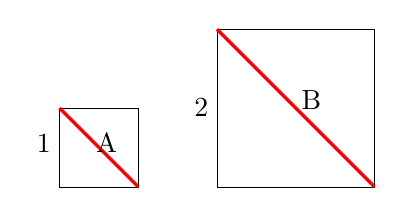
\begin{tikzpicture}
  \draw[very thin] (0,0) rectangle (1,1);
  \node at (-0.2,0.55) {1};
  \draw[very thick,red] (0,1) -- (1,0);
  \node at (0.60,0.55) {A};
  \draw[very thin] (2,0) rectangle (4,2);
  \node at (1.8,1) {2};
  \draw[very thick,red] (2,2) -- (4,0);
  \node at (3.2,1.1) {B};
\end{tikzpicture}
\caption{Diagonals of A 1x1 Square And A 2x2 Square}
\label{fig:1x12x2s}
\end{figure}
\pause
Are The Two \alert{Diagonals: A, B} Commensurable?
\pause
\begin{itemize}
\item If Not, Why Not?
\pause
\item If Yes, What Are The Common Unit And Whole Numbers for A, B?
\end{itemize}

\end{frame}


\begin{frame}
\frametitle{Commensurable Or Not?}
\begin{figure}[H]
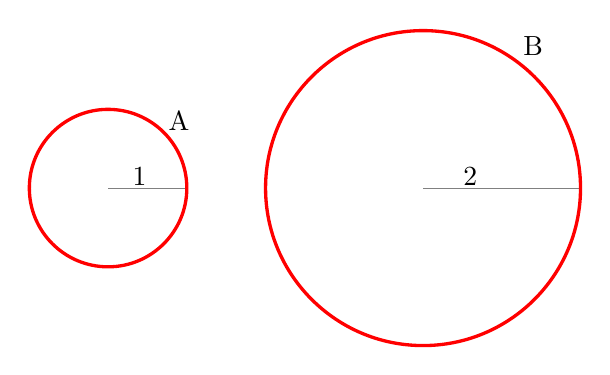
\begin{tikzpicture}
  \draw[very thin,gray] (0,0) -- (1,0);
  \node at (0.4,0.15) {1};
  \draw[very thick,red] (0,0) circle [radius=1cm];
  \node at (0.90,0.85) {A};
  \draw[very thin,gray] (4,0) -- (6,0);
  \node at (4.6,0.15) {2};
  \draw[very thick,red] (4,0) circle [radius=2cm];
  \node at (5.4,1.8) {B};
\end{tikzpicture}
\caption{Circumferences of Circles of Radii 1 and 2}
\label{fig:1c2c}
\end{figure}
\pause
Are The Two \alert{Circumferences A, B} Commensurable?
\pause
\begin{itemize}
\item If Not, Why Not?
\pause
\item If Yes, What Are The Common Unit And Whole Numbers for A, B?
\end{itemize}
\end{frame}

\begin{frame}
\frametitle{Integers}
\framesubtitle{They Are Special}
\label{slide:integers}
\begin{block}{Integers Are Natural}
God Made The Integers; All Else Is The Work of Man\footnote{The Mathematician Leopold Kronecker Said It First}.
\end{block}
\pause
\begin{itemize}
\item Do You Realize That Any Two Integers $A,B$ Are Commensurable?
\begin{itemize}
\pause
\item What Is the Common Unit?
\pause
\item What Are the Whole Numbers of $A,B$?
\end{itemize}
\end{itemize}
\end{frame}

\begin{frame}
\frametitle{One Fact About Incommensurable Magnitudes}
\framesubtitle{They Can Only Be Approximated}
\label{slide:incommensurablefact}
\begin{block}{Incommensurable Magnitudes Are Also Special}
\begin{itemize}
\pause
\item For Incommensurable Magnitudes, $A,B$, \alert{There Exists No Common Unit}!
\pause
\item That Means, When Expressed as A Ratio, There's Nothing Common in Them.
\pause
\item For Example, $\sqrt{2}$ Has \alert{No Exact Representation $\frac{A}{B}$}, Where $A, B$ Are Integers.
\begin{itemize}
\pause
\item Otherwise, as We've Seen, 1 Would Be A Common Unit.
\end{itemize}
\pause
\item That Means They Can Only Be \alert{Approximated as A Ratio of Two Integers: $\sqrt{2}\approx\frac{1414}{1000}$ Or $\sqrt{2}\approx\frac{14142}{10000}$}.
\begin{itemize}
\pause\item{\tiny That Funky Symbol $\approx$ Means \alert{Approximately Equals}}
\end{itemize}
\end{itemize}
\end{block}
\end{frame}

\begin{frame}
\frametitle{Modern Language}
\framesubtitle{We Build Our Math Vocabulary Using Previous Definitions}
\label{slide:modernlanguage}

Definition: Commensurable [\ref{def:commensurable}]
\pause
\begin{definition}[Rational Number]
If Magnitudes $A,B$ Are Commensurable,
Then
The Ratio $\frac{A}{B}$ Is Called 
\textit{A Rational Number}.
\end{definition}
\pause
\begin{definition}[Irrational Number]
If A Number is Not Rational, Then It Is \textit{Irrational}.
\pause

{\tiny Note: This Is a \textit{Negative} Definition. We Specify What Irrational Number Is Not.}
\end{definition}
\end{frame}

\begin{frame}
\frametitle{Our Vocabulary}
\framesubtitle{A Growing List of New Words And Symbols}
\label{slide:vocab}
\begin{itemize}
\pause
\item Commensurable.
\pause
\item Incommensurable.
\pause
\item Rational Number.
\pause
\item Irrational Number.
\pause
\item Integer.
\pause
\item Ratio.
\pause
\item Fraction, Numerator, Denominator\footnote{We Didn't Learn These Here, But Assumed That You Know These Words \dots}.
\pause
\item $\approx$: Approximately Equals.
\end{itemize}
\end{frame}




\begin{frame}
\frametitle{Commensurable Recap}

Was That Fun?
\pause

Is the Meaning of `Commensurable' Clearer Now?
\end{frame}

\begin{frame}
\frametitle{Does This Matter?}
\framesubtitle{There Are Definitions, Theorems, Proofs, Problems. Period.}
\label{slide:doesitmatter}
\begin{block}{It's A Matter of Perspective}
Perhaps None of This Matters.

Commensurable Magnitudes, Irrational Numbers, \dots Are All Meaningless Without The Fun.

Having Fun Matters.
\end{block}
\pause
\begin{block}{Let's Play Mindfully}
This Playful Introduction Is Meant to Be \dots
\pause

Well, Play!
\pause

Slowly, We Understand More, \pause And Play More!
\end{block}
\end{frame}

\begin{frame}
\frametitle{The Ever-Changing Magnitudes}
\framesubtitle{Things Change And That Changes Everything in Turn!}
\label{slide:changingmagnitudes}
\begin{itemize}
\item The Ever-Changing Universe Fascinates Us.
\pause
\item The Study of Changing, Rather Than Fixed, Magnitudes Fascinates Us.
\pause
\item Change Implies An Increase Or A Decrease.
\pause
\item Let's Start with The Ratio of Magnitudes That Are Capable of Changing \dots
\end{itemize}
\end{frame}


\begin{frame}
\frametitle{Ratio $r=\frac{A}{B}$}
\framesubtitle{Both $A$ and $B$ Can Change \dots}
\label{slide:abyb}
\begin{itemize}
\pause
\item Let's Play with Money! Let $A$ Represent Your Dollars and $B$ Mine.
\pause
\item Let's Say You Have $A=\$1$ And I $B=\$2$. 
\item $B-A=\$1$, $r=\frac{A}{B}=\frac{1}{2}$.
\pause
\item Which Is Right?
\begin{itemize}
\pause
\item I Have Much More Money Than You.
\item I Have Almost as Much Money as You.
\end{itemize}
\pause
\item Let's Say We Both Got $\$98$ (Things Changed!). You Now Have $\$99$ and I $\$100$. 
\item $B-A=\$1$, $r=\frac{A}{B}=\frac{99}{100}$.
\item Now Which Is Right?
\begin{itemize}
\pause
\item I Have Much More Money Than You.
\item I Have Almost as Much Money as You.
\end{itemize}
\end{itemize}
\end{frame}

\begin{frame}
\frametitle{Equality of Changing Quantities}
\framesubtitle{Their Difference Or Ratio?}
\label{slide:difforratio}
\begin{itemize}
\item Although in Both The Cases \dots 
\item The Difference $B-A=\$1$ Is The Same \dots
\pause
\item It's \alert{More Appropriate} To Say \dots
\item You And I Have \textit{Almost} The Same Money \alert{In the Second Case}.
\pause
\item It's \alert{More Appropriate} To Say \dots
\item You And I Have \textit{Almost} The Same Money \alert{When Their Ratio is Closer to 1}.
\pause
\item Therefore,
\item \alert{The Ratio, Not The Difference} Indicates \alert{The Equality of Changing Quantities}.
\pause
\item {\Large \alert{Do You Agree?}}
\end{itemize}
\end{frame}

\begin{frame}
\frametitle{Observation, Reflection, Analysis \dots}
\framesubtitle{Hypothesis, Thinking and Experimentation, Generalization \dots}
\label{slide:generalization}
\begin{itemize}
\item Let's Recap!
\pause
\item We Observe That 
\begin{itemize}
\pause
\item Two Quantities\footnote{Or Numbers, Magnitudes, Lengths, \dots}, Both Capable of Changing, \alert{Approach Each Other} \dots
\pause
\item When Their \alert{Ratio Approaches 1 \textit{Regardless} of Their Initial Difference}.
\end{itemize}
\pause
\item Is Our Observation Reliable Or Illusory?
\pause
\begin{itemize}
\item After All, We \alert{Only Tried One Case}: Increasing $A$ and $B$ by 98.
\end{itemize}
\item In Other Words, Does \alert{Our Observation Hold \textit{In General}?}
\end{itemize}
\end{frame}

\begin{frame}
\frametitle{Equality of Changing Quantities: Ratio or Difference?}
\framesubtitle{Everyday Language $\rightarrow$ Language of Math}
\label{slide:expressmath}
\begin{block}{Informally \dots}
We Want to Show That, In General, Two Different Magnitudes Approach Equality When Both Are Increased While Preserving The Difference.
\end{block}
\begin{itemize}
\pause
\item We Need to Be Precise.
\pause
\item But We Have Got to Start Somewhere and Proceed Logically.
\pause
\item We Use Symbols Or Notation for This Purpose.
\end{itemize}
\end{frame}

\begin{frame}
\frametitle{Equality of Changing Quantities: Ratio or Difference?}
\framesubtitle{Everyday Language $\rightarrow$ Language of Math}
\label{slide:expressmath2}
\begin{block}{Helpful Symbols?}
\begin{itemize}
\pause
\item Let $A,B$ \textit{Stand for} Initial Values of The Magnitudes.
\pause
\item Let $A<B$. In Other Words, $A$ \textit{Stands for} The Lesser of The Two Magnitudes.
\pause
\item Let $d$ \textit{Stand for} The Difference between $A,B$.
\pause
\begin{equation}
B=A+d
\end{equation}
\pause
\item Let $r$ \textit{Stand for} The Ratio of $A,B$.
\pause
\begin{equation}
r=\frac{A}{B} \pause\therefore r=\frac{A}{A+d}
\label{eq:newratio}
\end{equation}
\end{itemize}
\end{block}
\end{frame}

\begin{frame}
\frametitle{Equality of Changing Quantities: Ratio or Difference?}
\framesubtitle{Everyday Language $\rightarrow$ Language of Math}
\label{slide:expressmath3}
\begin{block}{Helpful Symbols? \dots}
\begin{itemize}
\item If The Magnitudes Increase Preserving Their Difference, $d$, Then
\pause
\item $A\rightarrow A+m$, $B\rightarrow B+m$ ({\tiny Right?})
\pause
\item {\tiny Where, $m$ \textit{Stands for} The Increase in Their Amount.}
\pause
\item What Does $r$ Now Become?
\pause
\begin{equation}
r\rightarrow\frac{A_{new}}{B_{new}}=\frac{A+m}{A+m+d}
\label{eq:newratio1}
\end{equation}
\pause
\item What Is The Question Now?
\pause
\item Right, \alert{Is $\frac{A+m}{A+m+d}$ Closer to 1 Than $\frac{A}{A+d}$?}\pause 

Given: $m$ Is A Positive Number (Because? \pause Right, We're \textit{Increasing} Magnitudes).
\end{itemize}
\end{block}
\end{frame}

\begin{frame}
\frametitle{Informally $\leftrightarrow$ Mathematically}
\framesubtitle{Speaking Math with Symbols \dots}
\label{slide:informalmathematical}
Translating between The Two \textit{Lingo}s:

\begin{columns}[t]
\column{.5\textwidth}
\begin{block}{Informally}
Two Different Magnitudes \alert{Approach Equality} When Both Are Increased While Preserving The Difference.
\end{block}
\pause
\column{.5\textwidth}
\begin{block}{Mathematically}
Which \alert{Ratio Is Closer to 1}? 

$r=\frac{A+m}{A+m+d}$ (Eq. [\ref{eq:newratio1}]) Or 

$r=\frac{A}{A+d}$ (Eq. [\ref{eq:newratio}])?

Given: $A<B, m>0$
\end{block}
\end{columns}
\begin{itemize}
\pause
\item Notice That The Translation \alert{Isn't Exact}.
\pause
\item ``Mathematically Speaking,'' We Clearly Specified Our Assumptions (\alert{e.g., $A<B$}).
\pause
\item Without Clarifying Assumptions, The Translation Fails!
\pause
\item Correct Translation Is An Art. Fortunately, Practice Makes Us Better!
\end{itemize}
\end{frame}

\begin{frame}
\frametitle{Which Is Closer to 1?}
\framesubtitle{How Will You Tell?}
\label{slide:whichiscloserto1}
Will You Analyze This Question Then?
\pause
\begin{block}{Mathematically}
Which \alert{Ratio Is Closer to 1}? 

$r=\frac{A+m}{A+m+d}$ (Eq. [\ref{eq:newratio1}]) Or 

$r=\frac{A}{A+d}$ (Eq. [\ref{eq:newratio}])?

Given: $A<B, m>0$
\end{block}
\pause
The Result of Your Analysis Will Be a \alert{Proof}.
\end{frame}

\begin{frame}
\frametitle{Mathematically Speaking}
\framesubtitle{And Proving}
\label{slide:whyspeakmathematically}

\begin{itemize}
\pause
\item
\alert{Proofs} Are The Way of Mathematics to Settle Questions Once And for All.
\pause
\item Once You Provide That Proof, The Truth Will Be Established (Under The Given Assumptions) Forever!
\end{itemize}
\end{frame}

\section*{Summary}
\begin{frame}
\frametitle{Summary of Chapter 1}
\framesubtitle{About Ratio of Changing Magnitudes}
\label{slide:summarych1}
\begin{block}{Changing Magnitudes}
\begin{itemize}
\pause
\item Commensurable Magnitudes (e.g. $2.5, 3.7$) Can Be Expressed As \alert{Exact Ratios} (e.g. \textit{Exactly} $\frac{25}{37}$).
\pause
\item Incommensurable Magnitudes (e.g. $\sqrt{3}, 2$) Can Only Be Approximated (e.g. \textit{Approximately} $\frac{866}{1000}$, or $\frac{86602}{100000}$).
\pause
\item Changing Magnitudes (\alert{Commensurable Or Incommensurable}) $A, B\;(A<B)$ Approach Equality When Increased While Keeping Their Initial Difference.
\end{itemize}
\end{block}
\end{frame}
% ------ copypasta next 5 ------
\begin{frame}
\frametitle{Frame Title}
\framesubtitle{Frame Subtitle}
\label{slide:slidelabel}
\end{frame}
% ------ copypasta prev 5 ------

\begin{comment}
\begin{frame}
\frametitle{There Is No Largest Prime Number}
\framesubtitle{The proof uses \textit{reductio ad absurdum}.}
\begin{theorem}
There is no largest prime number.
\end{theorem}
\begin{proof}
\begin{enumerate}
\item<1-> Suppose $p$ were the largest prime number.
\item<2-> Let $q$ be the product of the first $p$ numbers.
\item<3-> Then $q + 1$ is not divisible by any of them.
\item<1-> But $q + 1$ is greater than $1$, thus divisible by some prime
number not in the first $p$ numbers.\qedhere
\end{enumerate}
\end{proof}
\uncover<4->{The proof used \textit{reductio ad absurdum}.}
\end{frame}

\begin{frame}
\frametitle{What’s Still To Do?}
\begin{columns}[t]
\column{.5\textwidth}
\begin{block}{Answered Questions}
How many primes are there?
\end{block}
\pause
\column{.5\textwidth}
\begin{block}{Open Questions}
Is every even number the sum of two primes?
\cite{Goldbach1742}
\end{block}
\end{columns}
\end{frame}

\begin{thebibliography}{10}
\bibitem{Goldbach1742}[Goldbach, 1742]
Christian Goldbach.
\newblock A problem we should try to solve before the ISPN ’43 deadline,
\newblock \emph{Letter to Leonhard Euler}, 1742.
\end{thebibliography}

\end{comment}

%\begin{frame}{Learn from Masters} %{Subtitles are optional.}
%  % - A title should summarize the slide in an understandable fashion
%  %   for anyone how does not follow everything on the slide itself.
%
%  \begin{itemize}
%  \item
%    Use \texttt{itemize} a lot.
%  \item
%    Use very short sentences or short phrases.
%  \end{itemize}
%\end{frame}
%
%\begin{frame}{Make Titles Informative.}
%
%  You can create overlays\dots
%  \begin{itemize}
%  \item using the \texttt{pause} command:
%    \begin{itemize}
%    \item
%      First item.
%      \pause
%    \item    
%      Second item.
%    \end{itemize}
%  \item
%    using overlay specifications:
%    \begin{itemize}
%    \item<3->
%      First item.
%    \item<4->
%      Second item.
%    \end{itemize}
%  \item
%    using the general \texttt{uncover} command:
%    \begin{itemize}
%      \uncover<5->{\item
%        First item.}
%      \uncover<6->{\item
%        Second item.}
%    \end{itemize}
%  \end{itemize}
%\end{frame}
%
%
%\subsection{Second Subsection}
%
%\begin{frame}{Make Titles Informative.}
%\end{frame}
%
%\begin{frame}{Make Titles Informative.}
%\end{frame}
%
%
% [Kedar] Only one section in this presentation.
% [Kedar] No subsections, sections have slides.


\begin{comment}

\section*{Summary}

\begin{frame}{Summary}

  % Keep the summary *very short*.
  \begin{itemize}
  \item
    The \alert{first main message} of your talk in one or two lines.
  \item
    The \alert{second main message} of your talk in one or two lines.
  \item
    Perhaps a \alert{third message}, but not more than that.
  \end{itemize}
  
  % The following outlook is optional.
  \vskip0pt plus.5fill
  \begin{itemize}
  \item
    Outlook
    \begin{itemize}
    \item
      Something you haven't solved.
    \item
      Something else you haven't solved.
    \end{itemize}
  \end{itemize}
\end{frame}

\end{comment}

\end{document}


